\chapter{Evaluation and Analysis of GPU Communication}\label{eval}
This chapter analyses the traces generated with the technique described in chapter \ref{chap:impl}. The analysis is sectioned into several tiers, as described in \ref{methodik:methods}.\\


\section{Evaluated Applications}
The evaluated application are listed in table \ref{eval-apps}. The applications are selected to represent typical problem Domains in scientific computing. 
\begin{table}[h]
	\centering
\begin{tabular}{|l|c|c|c|c|}
	\hline 
	\textbf{Application} & \textbf{Source} & \textbf{Domain} & \textbf{Abbreviation} &\textbf{Problem Size} \\ 
	\hline 

%	\hline 
	Hotspot 2D & Rodinia & Structured Grid 2D & hs2d & 512x512, t = 10\\ 
%	\hline 
	Hotspot 3D & Rodinia & Structured Grid 3D & hs3d& 512x512x8, t = 10\\ 
%	\hline 
	Histogram64 & CUDA SDK & Histogram & hist& 64MB into 64 Bins\\ 
	NBody & ZiTi CEG & Nbody & nbody& 512 Bodies, t = 5\\ 
	Pathfinder & Rodinia & Shortest Path & path& 100000x100x20\\ 
%	\hline 
	Breadth First Seach & Rodinia & Graph Processing & bfs& $10^{6}$ Nodes\\ 
%	\hline 

	\hline 
\end{tabular} 
\caption{Application used for communication evaluation}
\label{eval-apps}
\end{table}
\textit{Hist}, \textit{hs2d}, \textit{hs3d} and \textit{nbody} are regular applications, where each CTA only operates within his data region. \textit{BFS} and \textit{path} contain irregularity, as the execution is  dynamic and the behaviour is depended on the input data.
\section{Tier I Analysis}
\subsection{Total Data Volume and Communication Fraction}
 Figure \ref{com-ratio} directly compares the total data volume of loads and stores of and how much of the write volume is involved in communication. At least 30\% of any application's writes is accessed by another CTA or another kernel in following iterations. As expected, loads exceed the stores by at least a single order of magnitude.

\textit{Nbody} and \textit{hist} show a very high ratio of communication, because \textit{nbody} is an $n$-to-$n$ problem and the histogram algorithm reduces a problem into bins, only using on the data generated in the preceding step. The irregular applications, \textit{bfs} and \textit{path}, communicate less data compared to the four regular applications.

Against initial expectations,  \textit{hs2d} and \textit{hs3d} show almost 50\% communication ration. The reason is, \textit{hs2d} uses deep halos which increase the number of transferred bytes between iterations. \textit{Hs3d} exchanges the complete $z$-dimension across iterations. 


\begin{figure}[t]
	\centering
	\includegraphics[width=\textwidth]{../../../Global-Memory-Tracing/memtrace-pass/plots/write-com-ratio}
	\caption{Total data volume and ratio of communication to total of all writes.}
	\label{com-ratio}
\end{figure}
\subsection{Transfer Size CDF}
Figure \ref{fig:CDF} shows the cumulative distribution functions (CDF) plots for each application. The CDF shows the cumulative probability of a transfer size between two CTAs to occur during the execution. All applications, except \textit{path}, show one or few dominating transfer sizes. The \textit{path} application shows two slopes with linear rising probability for a range of transfer sizes.

The dominant transfer size of \textit{bfs} is caused by the frontier array, used to communicate across graph segments. The \textit{hist} has one transfer size, because only one uniform kind of transfer happens in this application. This is also true for \textit{nbody}. The steps in \textit{hs2d} and \textit{hs3d} are caused by the problem space borders in the calculation

\begin{figure}[t]
%	\begin{subfigure}[b]{0.45\textwidth}
%		\includegraphics[width=1\linewidth]{../../../Global-Memory-Tracing/memtrace-pass/plots/cdf/bfs}
%		\caption{BFS}
%		\label{fig:cfd-bfs}
%	\end{subfigure}
%	\begin{subfigure}[b]{0.45\textwidth}
%		\includegraphics[width=1\linewidth]{../../../Global-Memory-Tracing/memtrace-pass/plots/cdf/hist}
%		\caption{Histogram}
%		\label{fig:density-hist}
%	\end{subfigure}
%	\begin{subfigure}[b]{0.45\textwidth}
%		\includegraphics[width=1\linewidth]{../../../Global-Memory-Tracing/memtrace-pass/plots/cdf/hs2d}
%		\caption{Hotspot 2D}
%		\label{fig:cfd-hs2d}
%	\end{subfigure}
%	\begin{subfigure}[b]{0.45\textwidth}
%		\includegraphics[width=1\linewidth]{../../../Global-Memory-Tracing/memtrace-pass/plots/cdf/hs3d}
%		\caption{Hotspot 3D}
%		\label{fig:cfd-hs3d}
%	\end{subfigure}
%	\begin{subfigure}[b]{0.45\textwidth}
%		\includegraphics[width=1\linewidth]{../../../Global-Memory-Tracing/memtrace-pass/plots/cdf/path}
%		\caption{Pathfinder}
%		\label{fig:cfd-path}
%	\end{subfigure}
%	%add desired spacing between images, e. g. ~, \quad, \qquad, \hfill etc. 
%	%(or a blank line to force the subfigure onto a new line)
%	\hfill
%	\begin{subfigure}[b]{0.45\textwidth}
%		\includegraphics[width=1\linewidth]{../../../Global-Memory-Tracing/memtrace-pass/plots/cdf/nbody}
%		\caption{NBody}
%		\label{fig:cfd-nbody}
%	\end{subfigure}
	\includegraphics[width=\textwidth]{../../../Global-Memory-Tracing/memtrace-pass/plots/combined-cfd}
	\caption{Message Size CDF Plots}
	\label{fig:CDF}
\end{figure}


\subsection{CTA In/Out-Degree}
The in and out degree describe the number  communication partners, separated between incoming and outgoing transfers, for each CTA. Figure \ref{fig:Cta-degree} plots the percentages of selected bins for each application. 

Except for \textit{nbody}, and to a smaller degree \textit{bfs} and \textit{path}, no application performs point-to-point communication. Almost every communication happening is, to some degree, a collective communication.

Most applications show low variance of in- and out-degree, and few communication partners. \textit{Bfs} has a high variation because the traversed graphs dictates the communication partners. The partners of \textit{hs2d} are a result of 2D tiling and \textit{hs3d}s partners
dictated by stencil size. Also notable is that although \textit{path} is a dynamic application, the number of communication partners is steady. The in/out-degree of \textit{hist} stems from the two-step process, where each CTA in the second step reads a value from
every CA in the first step.

\begin{figure}[t]
	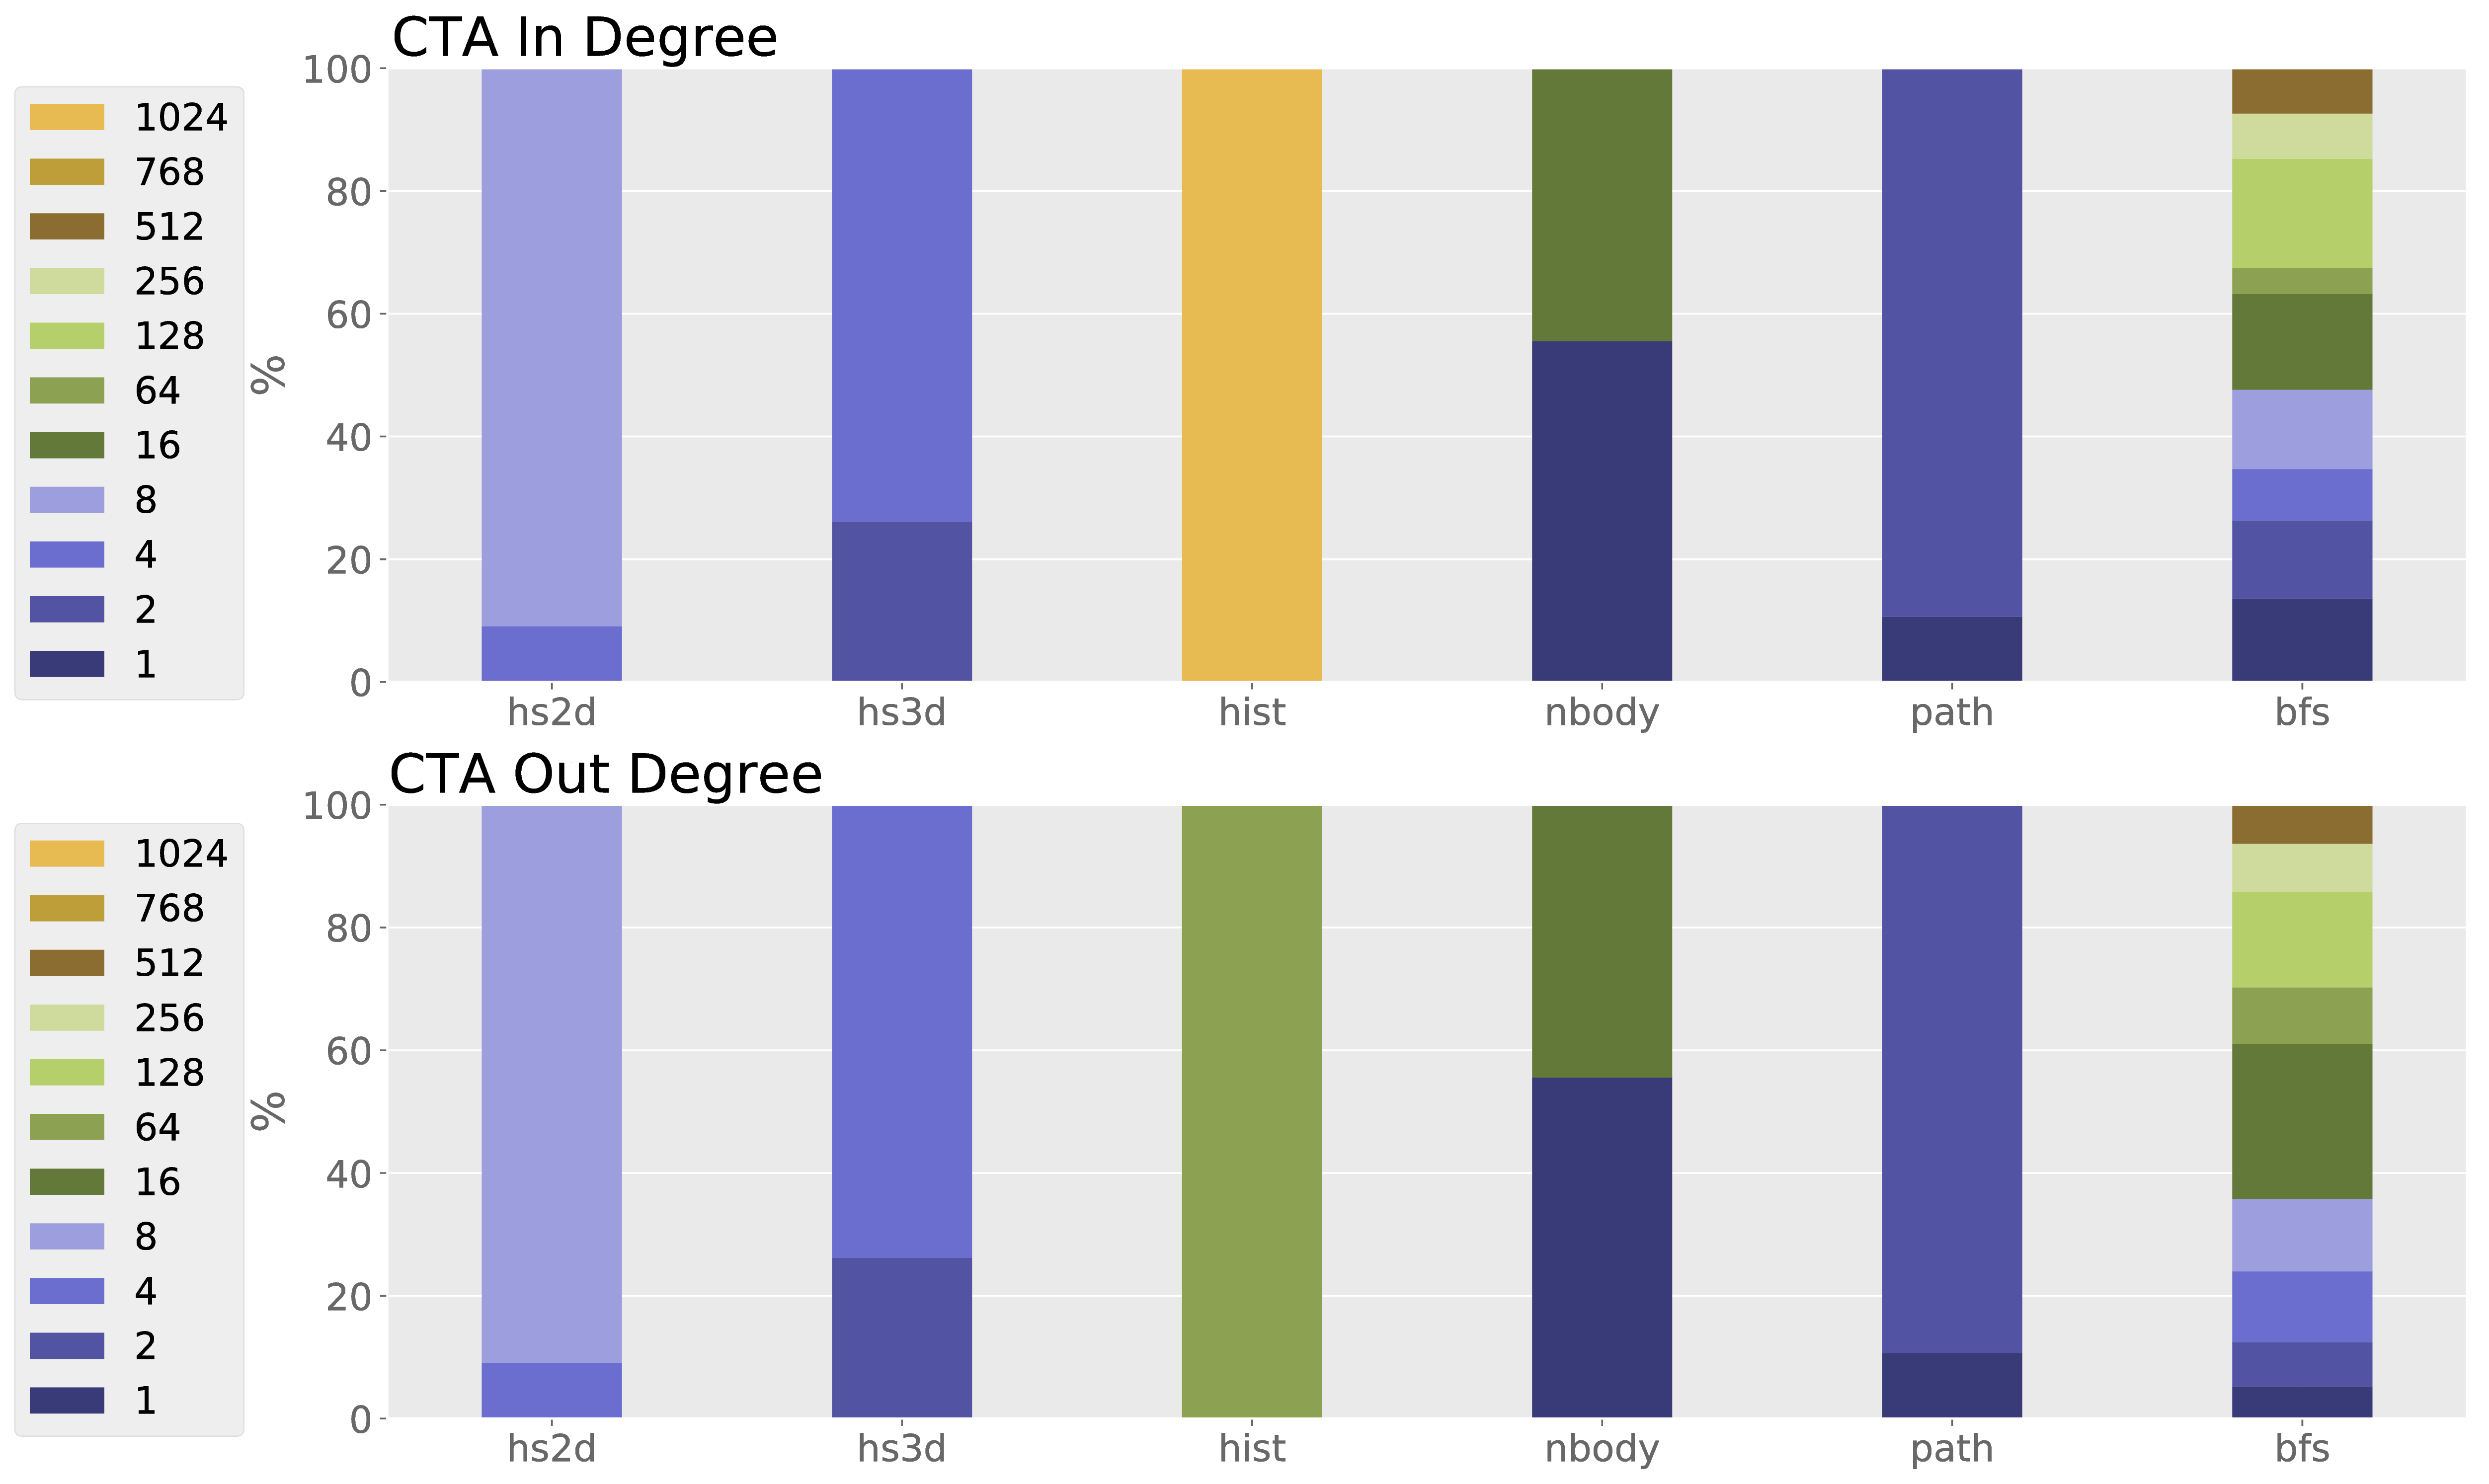
\includegraphics[width=\textwidth]{../../../Global-Memory-Tracing/memtrace-pass/plots/cta-degree}
	\caption{Number of incoming and outgoing communication partners of each CTA}
	\label{fig:Cta-degree}
\end{figure}
\subsection{Bisection Volume}
This metric shows the data volume moved a hypothetical cut in each dimension. The cut creates two equally sized grids. This can help analyse, how well an application scales to multiple GPUs. Because none of analysed application use the $z$-dimension of CTA organisation, only the $x$ and $y$ dimensions are plotted. 

\textit{Hs3d} strikes out, as it clearly shows that a cut in the $y$-dimension would not be favourable. The path algorithm shows a very low bisection volume, making it a good candidate for multi-gpu scaling.
Because of \textit{bfs} very irregular access patterns and high bisection volume and ratio, scaling to multiple GPUs can be challenging. The same goes for \textit{hist} and \textit{nbody}, because they both
perform all-to all communication. The scalability of the stencil applications depends on the problem, stencil and halo size and halo.
\begin{figure}[t]
	\centering
	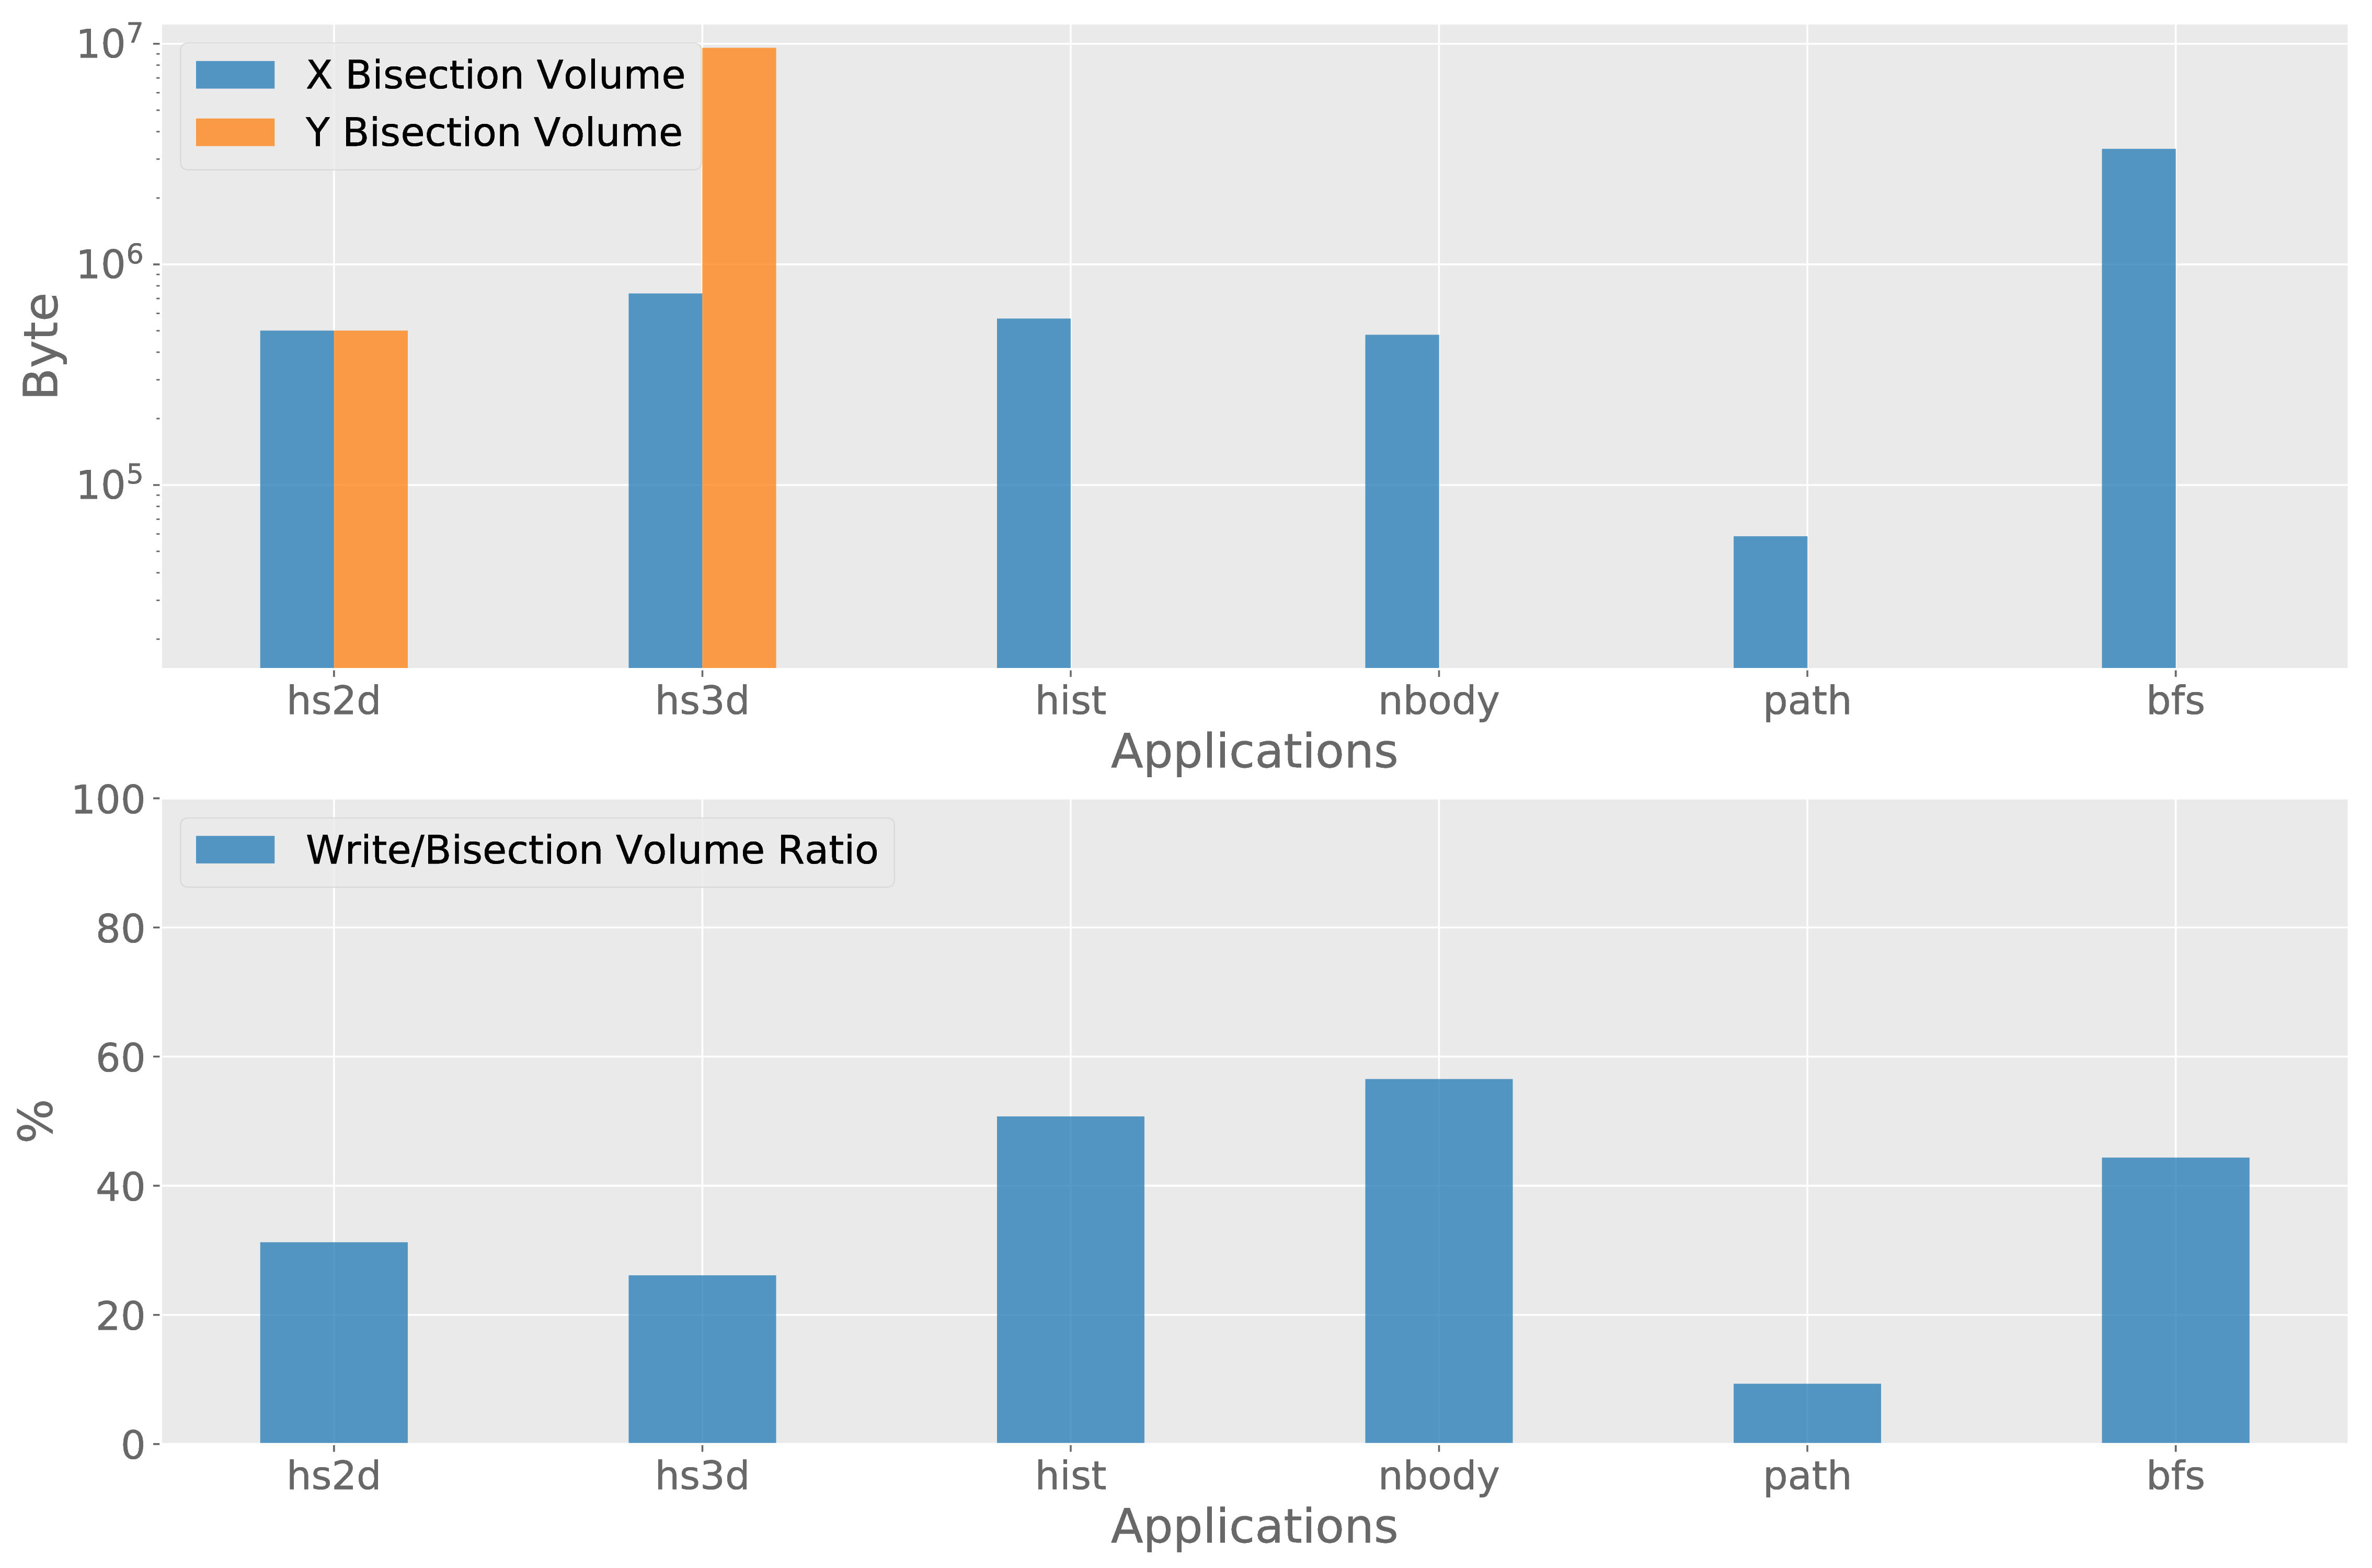
\includegraphics[width=\textwidth]{../../../Global-Memory-Tracing/memtrace-pass/plots/bisection-volume}
	\caption{Total and relative bisection Volume, separated by dimensions}
	\label{bisection-vols}
\end{figure}
\subsection{Communication Stride}
The stride in loads and stores involved in communication can be a critical aspect for performance. Large strides reduce the available memory bandwidth and increase latency. The strides in figure \ref{com-stride} are measured in byte distance, not elements.

The \textit{hist} application shows a large load stride in figure \ref{com-stride}, together with a large in-degree in figure \ref{fig:Cta-degree} suggest a 'gather'-like characteristic. For \textit{hs2d}/\textit{hs3d} we see the expected stride created by the tiling/stencil, accessing multiple rows at once.
The irregular pattern of \textit{bfs} is caused by the frontier array, which is used to communicate between all CTAs. The stride of nbody
is
\begin{figure}[t]
	\centering
	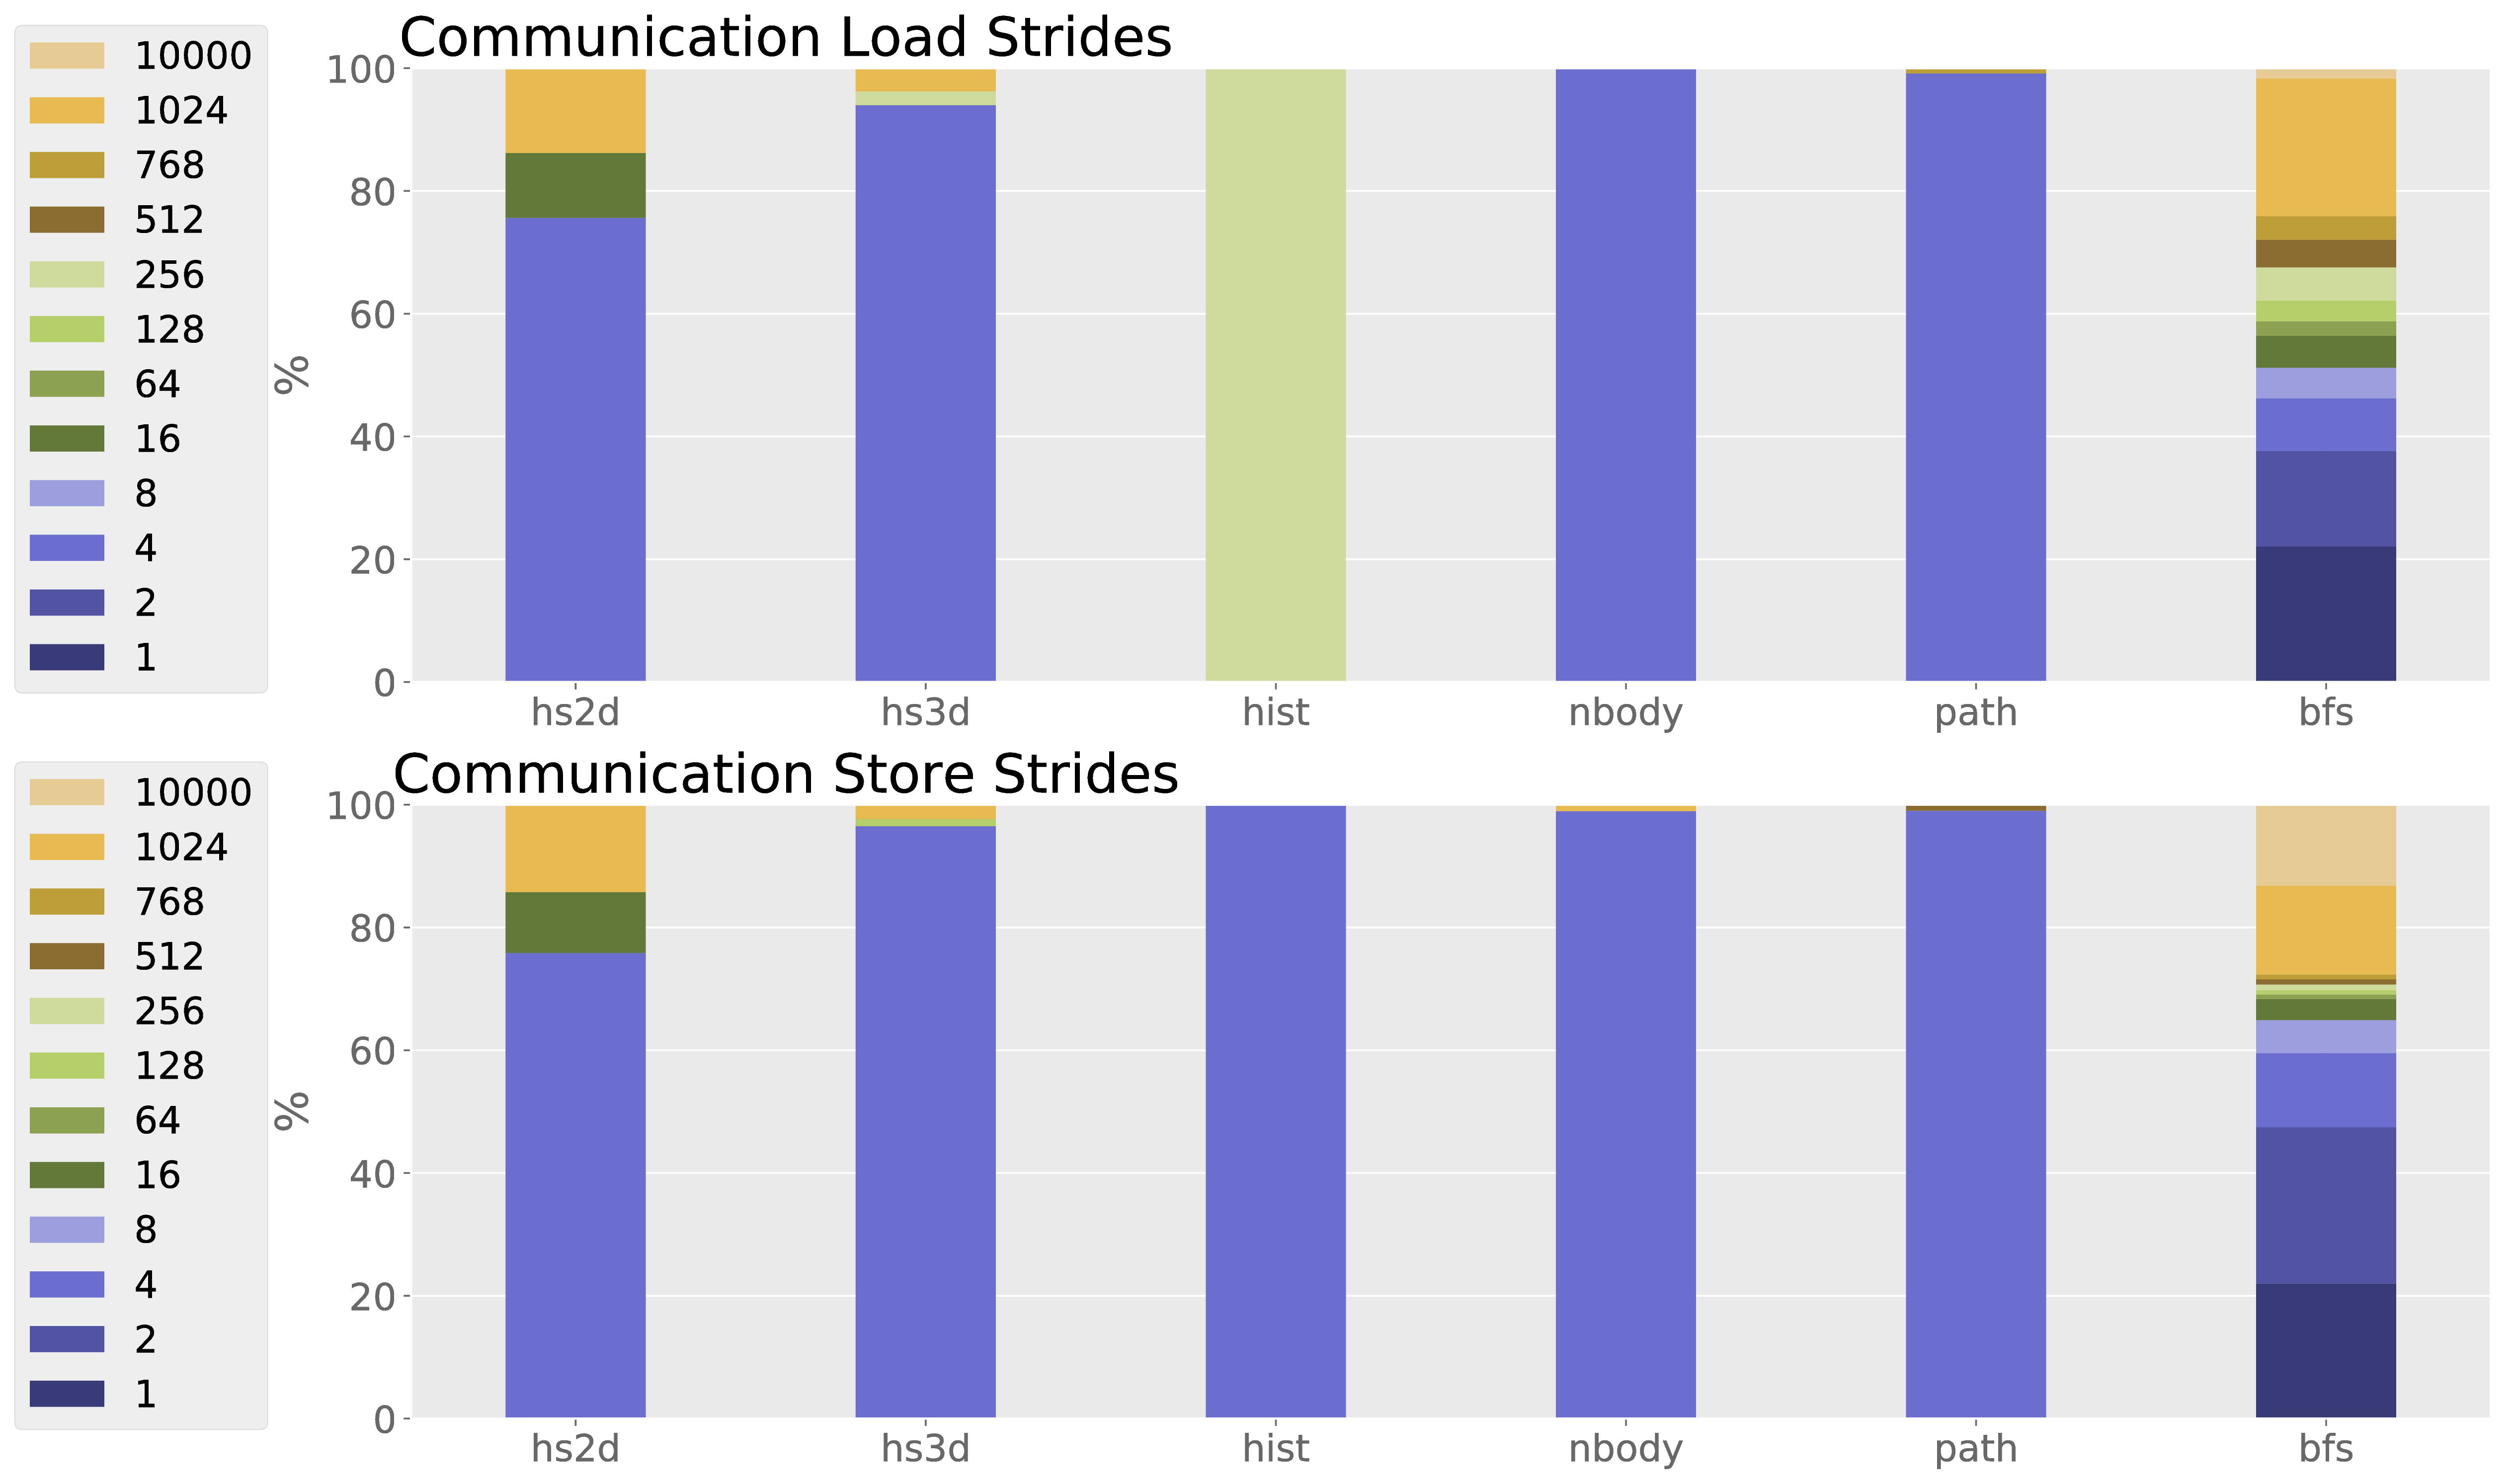
\includegraphics[width=\textwidth]{../../../Global-Memory-Tracing/memtrace-pass/plots/strides}
	\caption{Strides of loads and stores used in communication, by CTA}
	\label{com-stride}
\end{figure}
\subsection{Density Map}
The density plots, sometimes called heatmap, describes the frequency of CTA interaction across BSP supersteps. The x-axis are the CTAs performing writes, the y-axis are the follow-up reads to each write. Different kernels in an application are ignored, and only the CTA ID is used to identify communciation partners. Figure \ref{fig:density-plots} displays a subset of 200 CTAs for each application. The IDs of all CTA are serialized in $x$,$y$,$z$ order, $x$ being the most dominant dimension. 

The regular application show the expected patters. The stencils show communication with their neighbours according to stencil and tiling, \textit{nbody} shows communication with all other CTAs, same as \textit{hist}.

The irregular applications show two very different patters. \textit{Path} has only few partners but the frequency varies significantly. \textit{Bfs} shows two extremes, high frequency with high regularity and low frequency with low regularity.
The first extreme is caused by two kernels alternating during the iterations, where CTAs with the same ID process the same segment of the graph.  Latter is caused by the frontier array, used at the segment borders. A different graph would create the same pattern of the first extreme, but a different pattern of the second extreme.

The \textit{nbody} plot does not show 200 CTAs, as it only used 15 CTAs.

As the CDF plot shows, all applications are dominated by few transfer sizes between CTAs, the patterns in figure \ref{fig:density-plots} would remain largely unchanged if the density was replaced with accumulated data volumes.
\begin{figure}[h!]
	\begin{subfigure}[b]{0.45\textwidth}
		\includegraphics[width=1\linewidth]{../../../Global-Memory-Tracing/memtrace-pass/plots/heatmap/bfs}
		\caption{BFS}
		\label{fig:density-bfs}
	\end{subfigure}
	\begin{subfigure}[b]{0.45\textwidth}
		\includegraphics[width=1\linewidth]{../../../Global-Memory-Tracing/memtrace-pass/plots/heatmap/hist}
		\caption{Histogram}
		\label{fig:density-hist}
	\end{subfigure}
	\begin{subfigure}[b]{0.45\textwidth}
		\includegraphics[width=1\linewidth]{../../../Global-Memory-Tracing/memtrace-pass/plots/heatmap/hs2d}
		\caption{Hotspot 2D}
		\label{fig:density-hs2d}
	\end{subfigure}
	\begin{subfigure}[b]{0.45\textwidth}
		\includegraphics[width=1\linewidth]{../../../Global-Memory-Tracing/memtrace-pass/plots/heatmap/hs3d}
		\caption{Hotspot 3D}
		\label{fig:density-hs3d}
	\end{subfigure}
	\begin{subfigure}[b]{0.45\textwidth}
		\includegraphics[width=1\linewidth]{../../../Global-Memory-Tracing/memtrace-pass/plots/heatmap/path}
		\caption{Pathfinder}
		\label{fig:density-path}
	\end{subfigure}
	%add desired spacing between images, e. g. ~, \quad, \qquad, \hfill etc. 
	%(or a blank line to force the subfigure onto a new line)
	\hfill
	\begin{subfigure}[b]{0.45\textwidth}
		\includegraphics[width=1\linewidth]{../../../Global-Memory-Tracing/memtrace-pass/plots/heatmap/nbody}
		\caption{NBody}
		\label{fig:density-nbody}
	\end{subfigure}
	\caption{Transfer Density Plots}
	\label{fig:density-plots}
\end{figure}
\\\\\\\\\
\section{Tier II Analysis}
\subsection{Kernel communication Evolution}
This analysis if figure \ref{trans-ratio} shows how the data volumes change across supersteps. It is separated into loads and stores. Loads start at superstep one because as to our definition of communication, there can be no load that is part
of communication during the first superstep. Stores are not displayed in the last iteration, because the last store of an application is no communication.

The graph is to read as such: Stores happened in this superstep and are readable in the next. Loads read data from the preceding superstep. CTA in- and out degree analysis showed, every communication is happening in a collective environment. This means that there is no simple single writer, single reader matching across supersteps, which is the reason loads and stores are separated in this graphs.

As expects, the data of all regular applications follow a pattern, while the ones on irregular applications do not. The stencils do not
vary volumes, because every iteration performs exactly the same task. Because each CTA only updates
it's own set of bodies, \textit{nbody} has constant store volumes. The load volume of every other iteration accesses all bodies, creating the zig-zag pattern.
\begin{figure}[h!]
	\centering
	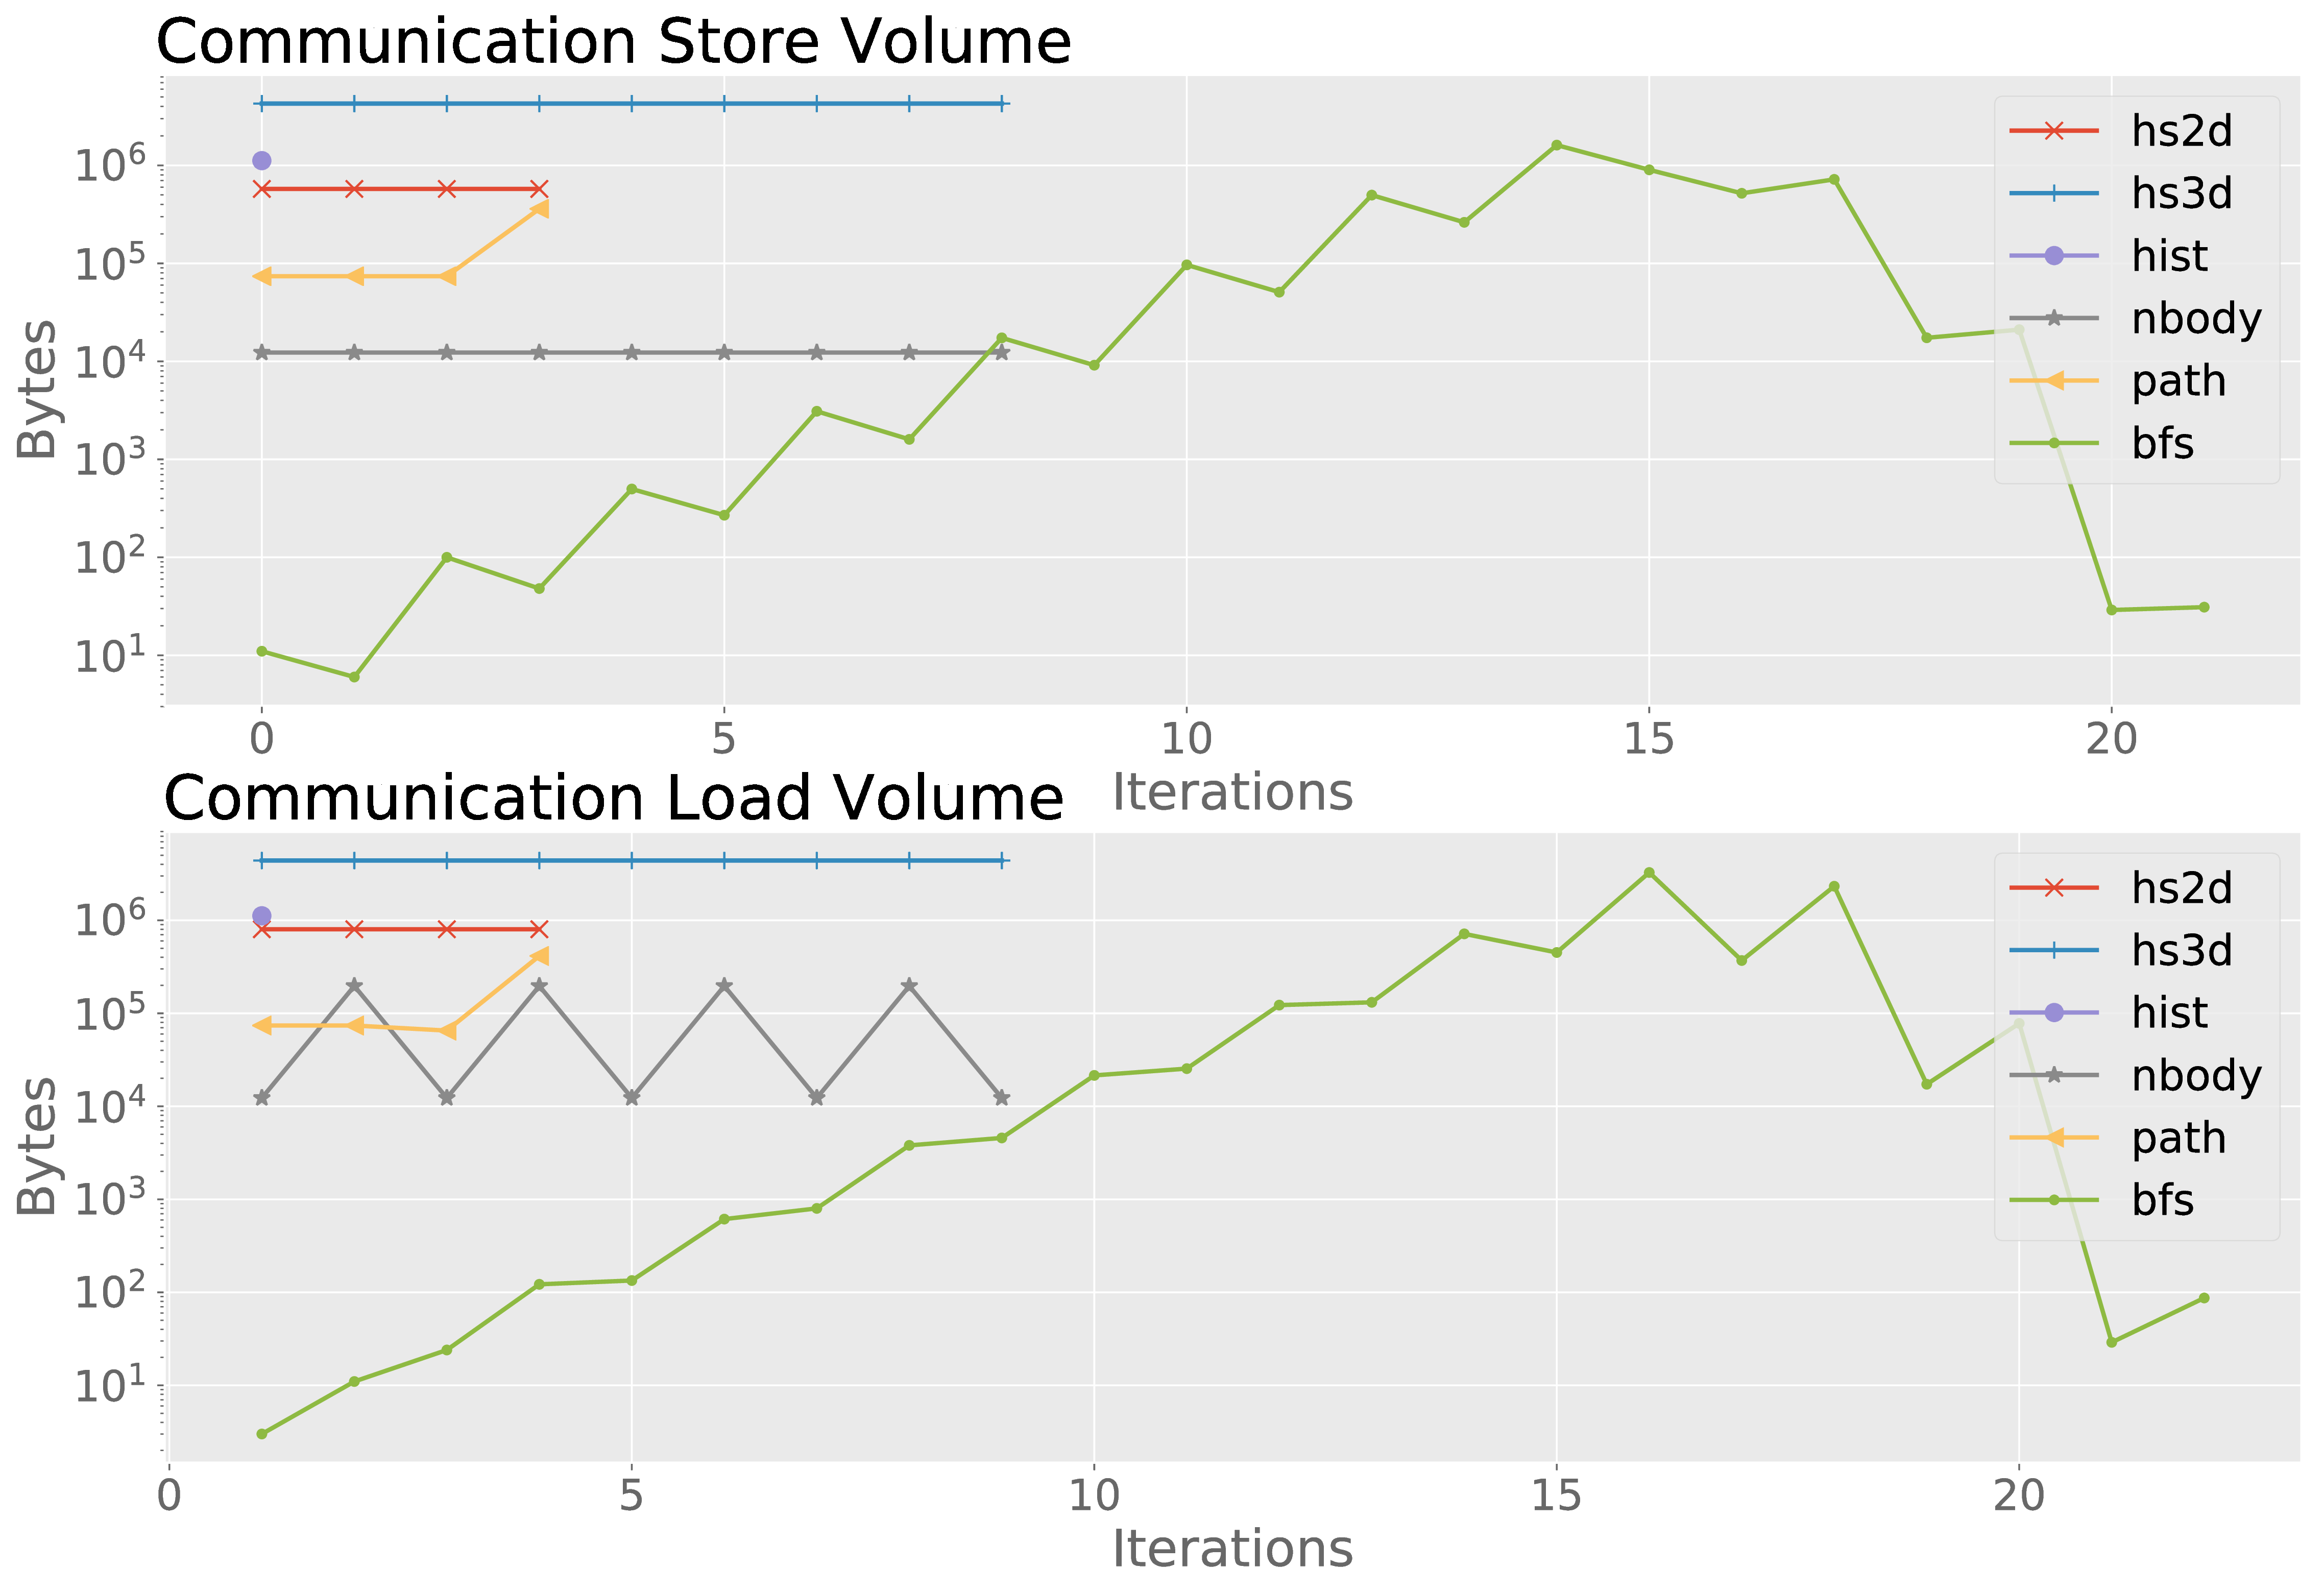
\includegraphics[width=\textwidth]{../../../Global-Memory-Tracing/memtrace-pass/plots/transmission-ratio}
	\caption{Volume of communication loads and stores in each iteration}
	\label{trans-ratio}
\end{figure}
\subsection{Superstep Distance}
This metric measures the volume of data transferred, but takes into account the number of supersteps distance between the store and the subsequent load. Only \textit{bfs} shows this behaviour,
figure \ref{trans-distance} shows only the volume for this application. The distance describes the number
of supersteps, or kernel launches, happening before written data is read by a CTA. A distance of zero means, the directly succeeding kernel reads the data.

Read operations in different supersteps can reference the same write, therefore the volumes are not exclusive.
As an example, a subset of distance zero might very well be included in more distant reads.
\begin{figure}[t]
	\centering
	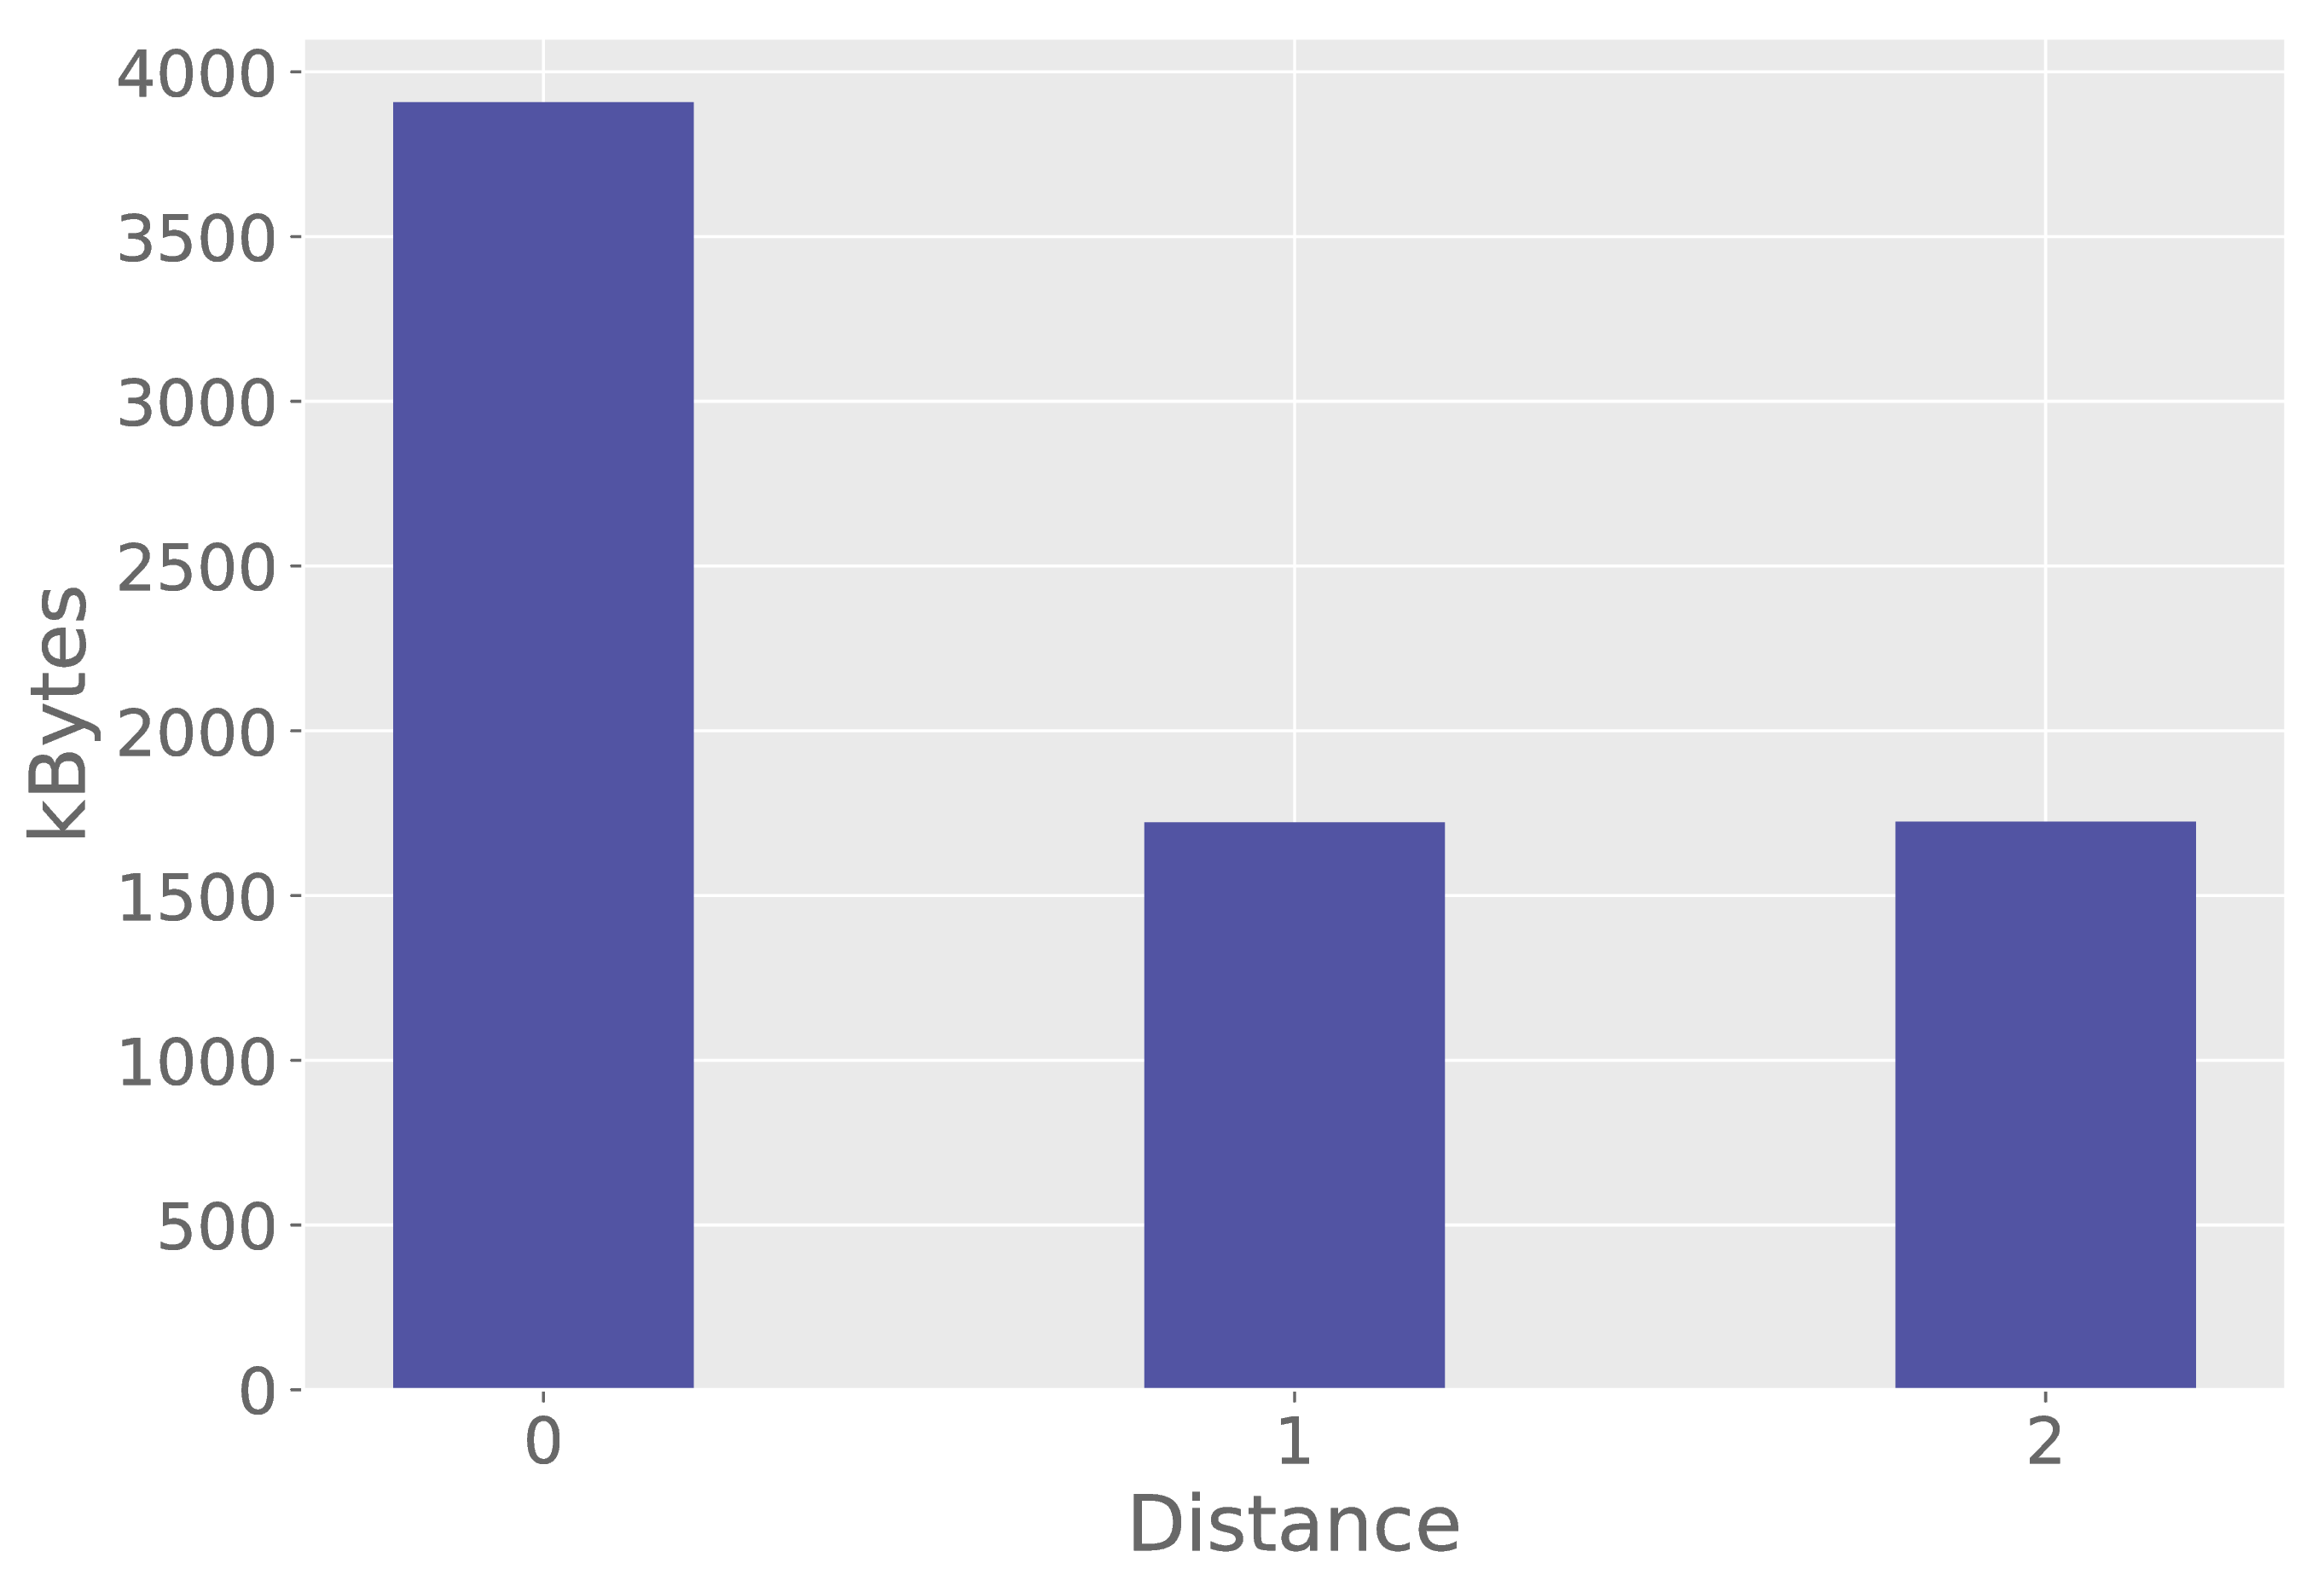
\includegraphics[height=0.3\textheight]{../../../Global-Memory-Tracing/memtrace-pass/plots/distances}
	\caption{Volume of communication for \textit{bfs} application, separated by superstep distance.}
	\label{trans-distance}
\end{figure}
\section{Tier III Analysis}

\subsection{CTA connectivity evolution}
As shown in figure \ref{fig:Cta-degree}, most applications have a steady number incoming and outgoing connections. Figure \ref{philandering} shows how the mean number of outgoing communication partners changes over time, including the standard deviation. 

The large fluctuation of \textit{nbody} can be explained with two alternating kernels, one kernel accesses only it's own set of bodies, while the other kernel accesses all bodies, which increases the out-degree. Because \textit{hist} consists of only two steps, it is represented by single value. Both \textit{path} and \textit{bfs} show stronger fluctuations with increasing number of iteration, caused by the exploration of the graph. Same as with the load and store volume of each iteration, the stencils show no variation.

\begin{figure}[h!]
	\centering
		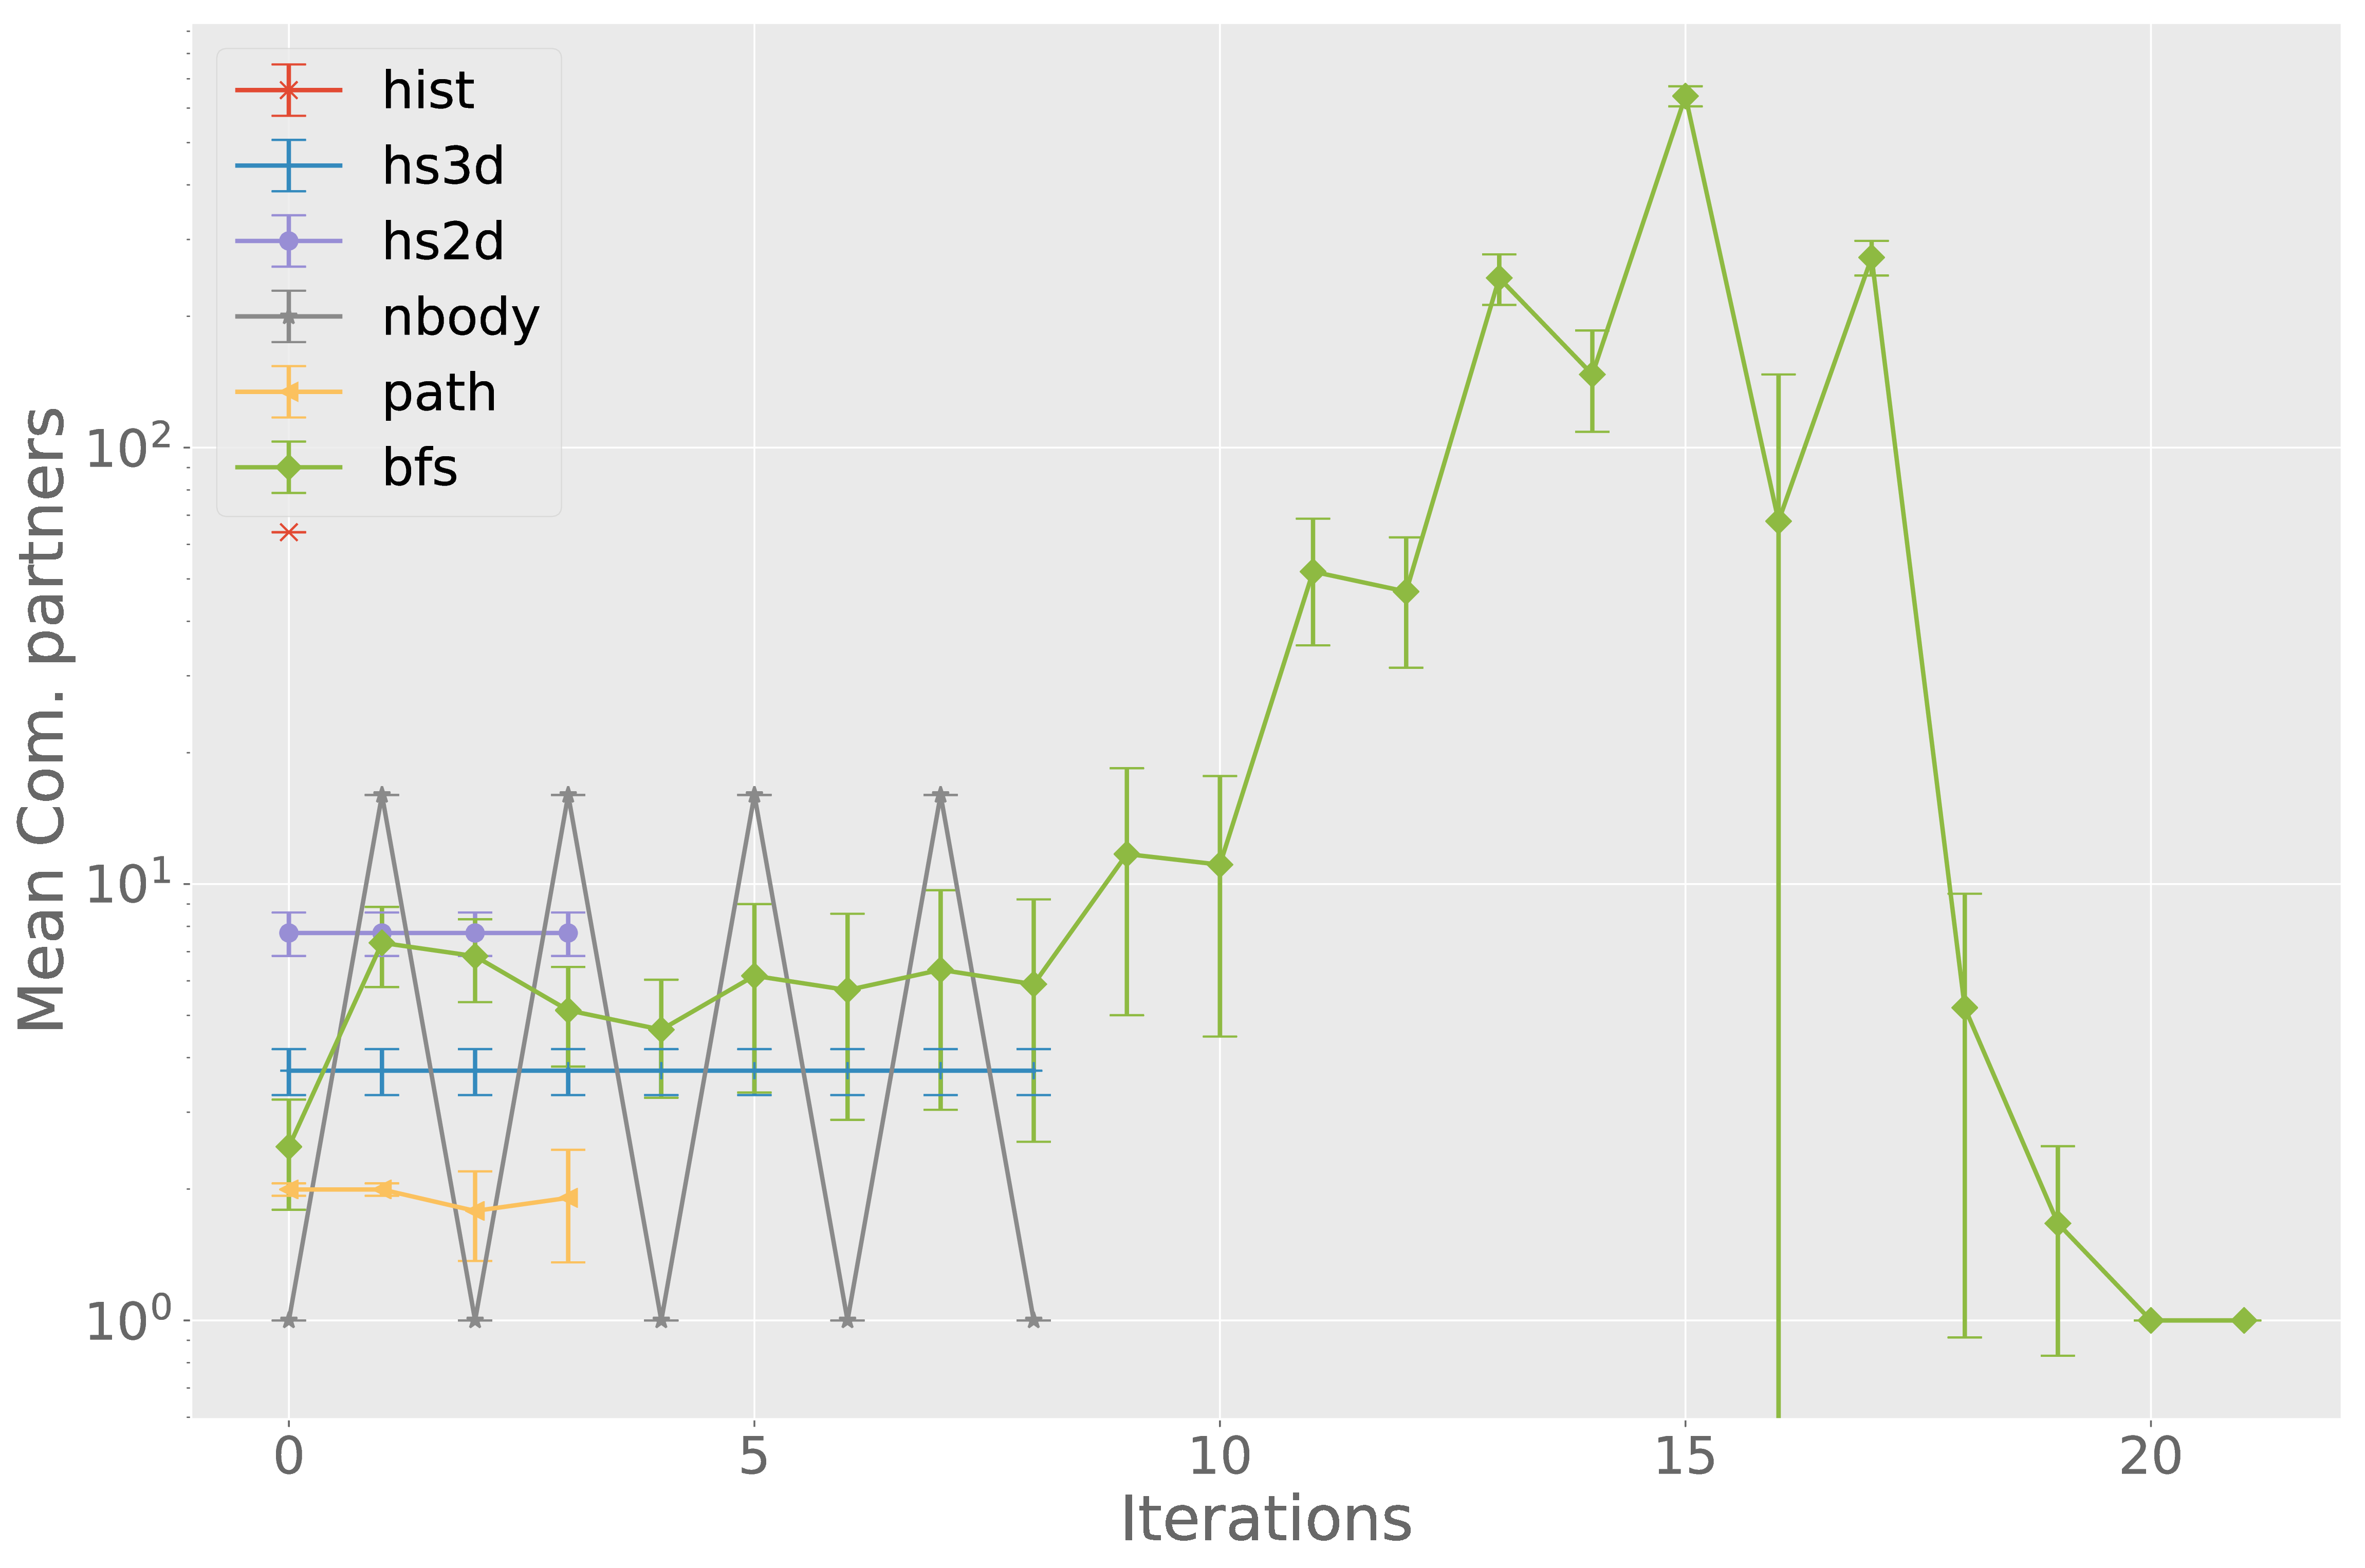
\includegraphics[width=\textwidth]{../../../Global-Memory-Tracing/memtrace-pass/plots/transmission-regularity}
	\caption{Mean out-degree of CTAs, per iteration}
	\label{philandering}
\end{figure}